\documentclass[border=6pt]{standalone}
\usepackage{amsmath}
\usepackage{tikz}
\usepackage{pgfplots}
\pgfplotsset{compat=1.18}
\usetikzlibrary{arrows.meta,calc,positioning}
\begin{document}
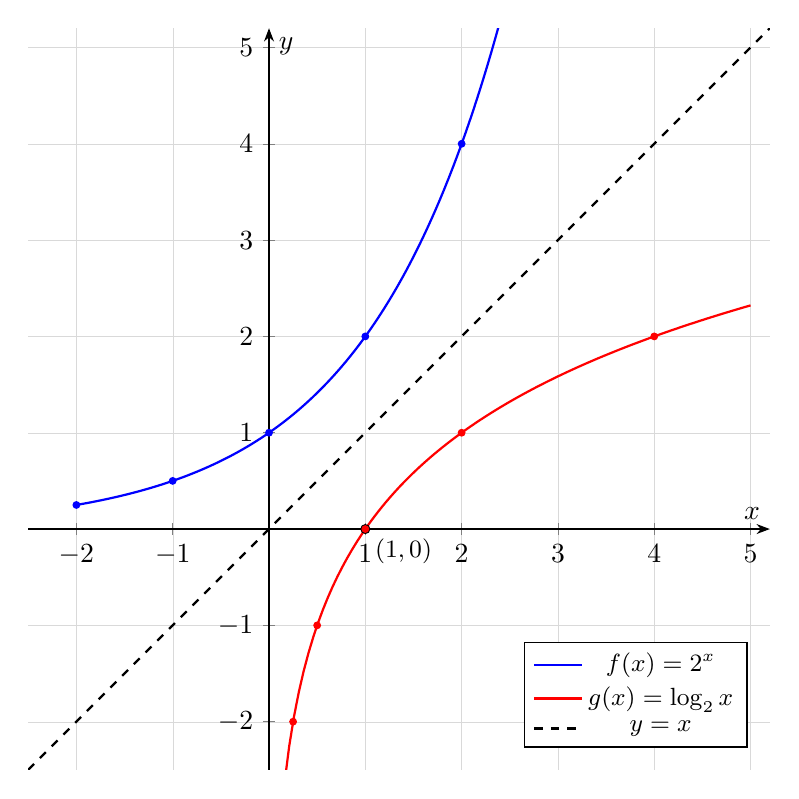
\begin{tikzpicture}
\begin{axis}[
    axis lines = middle,
    xlabel = {$x$}, ylabel = {$y$},
    xmin=-2.5, xmax=5.2, ymin=-2.5, ymax=5.2,
    xtick={-2,-1,0,1,2,3,4,5},
    ytick={-2,-1,0,1,2,3,4,5},
    grid=both,
    grid style={line width=.1pt, draw=gray!30},
    width=11cm, height=11cm,
    axis line style={-Stealth},
    legend pos=south east,
    legend style={font=\small},
]
% f(x) = 2^x , domain roughly x in [-2,5]
\addplot[domain=-2:2.4, samples=100, thick, blue] {2^x};
\addlegendentry{$f(x)=2^x$}

% g(x) = log_2(x), domain x>0
\addplot[domain=0.06:5, samples=100, thick, red] {ln(x)/ln(2)};
\addlegendentry{$g(x)=\log_2 x$}

% y = x reflection line, dashed
\addplot[domain=-2.5:5.2, samples=2, dashed, black, thick] {x};
\addlegendentry{$y=x$}

% vertical asymptote of g at x=0 (the y-axis itself already shown)
% mark x-intercept of g at (1,0)
\addplot[only marks, mark=*, mark size=1.6pt, black] coordinates {(1,0)};
\node[anchor=north west] at (axis cs:1,0) {\small $(1,0)$};

% key points for f
\addplot[only marks, mark=*, mark size=1.2pt, blue] coordinates {(-2,0.25) (-1,0.5) (0,1) (1,2) (2,4)};
% key points for g
\addplot[only marks, mark=*, mark size=1.2pt, red] coordinates {(0.25,-2) (0.5,-1) (1,0) (2,1) (4,2)};

\end{axis}
\end{tikzpicture}
\end{document}
